\documentclass{article}
\usepackage{hyperref}
\usepackage[normalem]{ulem}
\usepackage{moreverb}
\usepackage{color}
\usepackage{amsmath}
\usepackage{listings}
\usepackage{graphicx}
\usepackage[top=2cm, bottom=2cm, left=2cm, right=2cm]{geometry}
\usepackage{multirow}
\usepackage{amsfonts}
\usepackage{tabularx}
\usepackage{fancyvrb}
\usepackage{algorithm}
\usepackage{algpseudocode}
\let\subsubsubsection\paragraph
\let\subsubsubsubsection\subparagraph
\lstset{breaklines=true, breakatwhitespace=true, captionpos=b, tabsize=3, showtabs=false, numbers=left, frame=single, firstnumber=1}
\usepackage[english]{babel}

\lstdefinelanguage{JavaScript}{
  keywords={break, case, catch, continue, debugger, default, delete, do, else, finally, for, function, if, in, instanceof, new, return, switch, this, throw, try, typeof, var, void, while, with, cross, minus, belongsTo,true,false, let, foreach, union, emptySet},
  morecomment=[l]{//},
  morecomment=[s]{/*}{*/},
  morestring=[b]',
  morestring=[b]",
  sensitive=true
} % http://tex.stackexchange.com/posts/95460/revisions

\begin{document}
\tableofcontents
\begin{sloppypar}

\section{Introduction}
% Putting the Automata Theory Withing Reach

\paragraph{}
Teaching abstract concepts is only possible if these concepts are put within student's reach. There are multiple ways to do this and each teacher has its own approach, as well as each student is more sensitive to some ways of knowledge transmission than to other ways. Some students might be more sensitive to the structure of the speech and the mathematical robustness of definitions, some might be more likely to assimilate knowledge if they can hear a teacher explain it, some might need to visualize concepts with their eyes, some might need a mix of several ways and the more ways are exploited to transmit things, the more student should be involved in the knowledge transmission as these ways are more complementary than redundant.


\paragraph{}
Teachers who are eager to maximize the number of ways they take to transmit knowledge might be interested in making abstract concepts visualizable, dynamic therefore adding a concrete aspect of the concepts. The goal of the tool is to put the automata theory in student's hands, making it manipulable (``hackable'').

\section{Features of the tool}
\subsection{Drawing automata}


\paragraph{}
One of the needed feature to automata manipulation is being able to input them in a convenient way and like other tools of the domain, the tool provides a means to input automata by drawing them with the mouse and the keyboard in a hopefully intuitive way. For student who want to go farther, for repetitive tasks or big automata, the tool provides a way to write automata using a concise language instead of drawing them.


\paragraph{}
To display results of algorithms or automata which were written rather than drawn, the tool embeds a Javascript version\footnote{Viz.js: \href{https://github.com/mdaines/viz.js/}{https://github.com/mdaines/viz.js/}} of Graphviz\footnote{\href{http://www.graphviz.org/}{http://www.graphviz.org/}} to render graphical version of automata automatically.


\paragraph{}
To help writing documents about automata, the tool provides a way to export images or DOT\footnote{\href{http://www.graphviz.org/content/dot-language}{http://www.graphviz.org/content/dot-language}} codes of automata produced by the user or the tool. DOT documents can then be translated into TiKZ\footnote{\href{http://www.ctan.org/tex-archive/graphics/pgf/}{http://www.ctan.org/tex-archive/graphics/pgf/}} format in order to include automata in a LaTeX document.


\subsection{Algorithms}


\paragraph{}
So as to let students experiment with automata-related algorithm, the tool embeds a custom programming language and some common algorithms written in this language especially designed for manipulating sets and automata (see figure \ref{aude-algo}). With this possibility of testing algorithms of the lesson, of reading and implementing them without worrying about sets implementation, automata-related algorithms are made more experiencible for students. This language, named Audescript, is a customized Javacript which ease set manipulations with a notation for writing sets and set operators. Its also provides a means to specify types on variables.


\paragraph{}
The tool comes with some basic algorithms such as:

\begin{itemize}
   \item{determinization: get a determinist automaton from any automaton.}
   \item{completion: get a complete automaton from any automaton.}
   \item{minimization: get a minimal automaton from any automaton.}
   \item{epsilon removal: get an automaton without any epsilon transition from any automaton.}
   \item{product: get an automaton which recognize the intersection of the two input automata's respective languages.}
   \item{equivalence: test whether two automata recognize the same language.}
   \item{complementation: get an automaton which recognize the complementary language of the input automaton.}
   \item{empty and infinite language tests: test whether an automaton recognize the empty language and an infinite language, respectively}
   \item{regular expression to automaton: get an automaton recognizing the language described by a regular expression.}
\end{itemize}
\begin{figure}[htb]\centering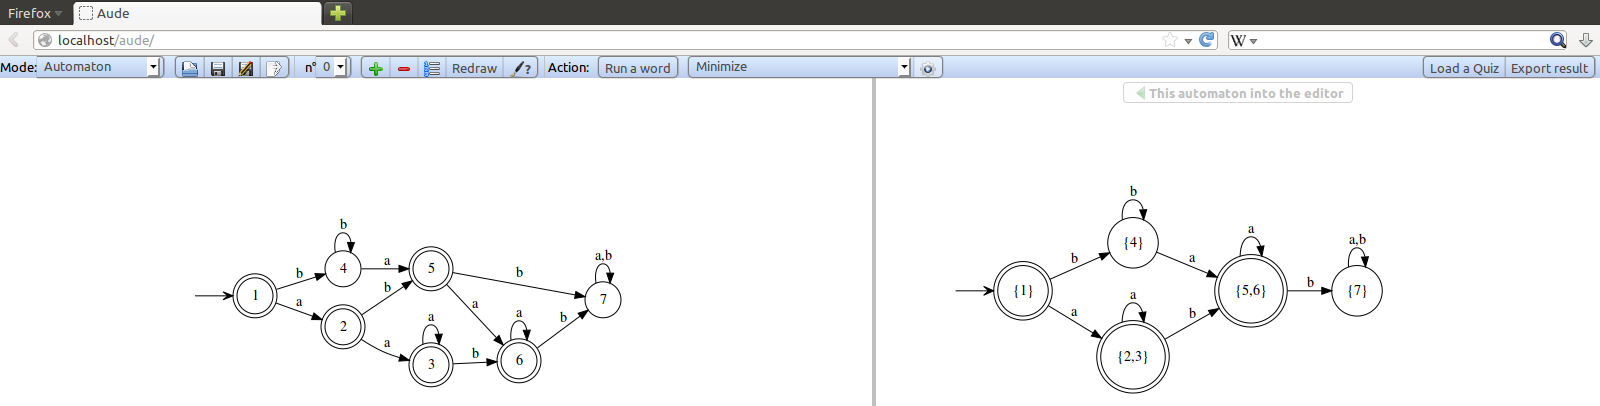
\includegraphics[width=500pt]{{../aude-algo}.png}\caption{Result of an algorithm execution.}\label{aude-algo}\end{figure}


\newpage

\paragraph{}
In addition, students can write their own algorithms using the same dedicated language as the one used for writing embedded algorithms (See figure \ref{aude-prog}).

\begin{figure}[htb]\centering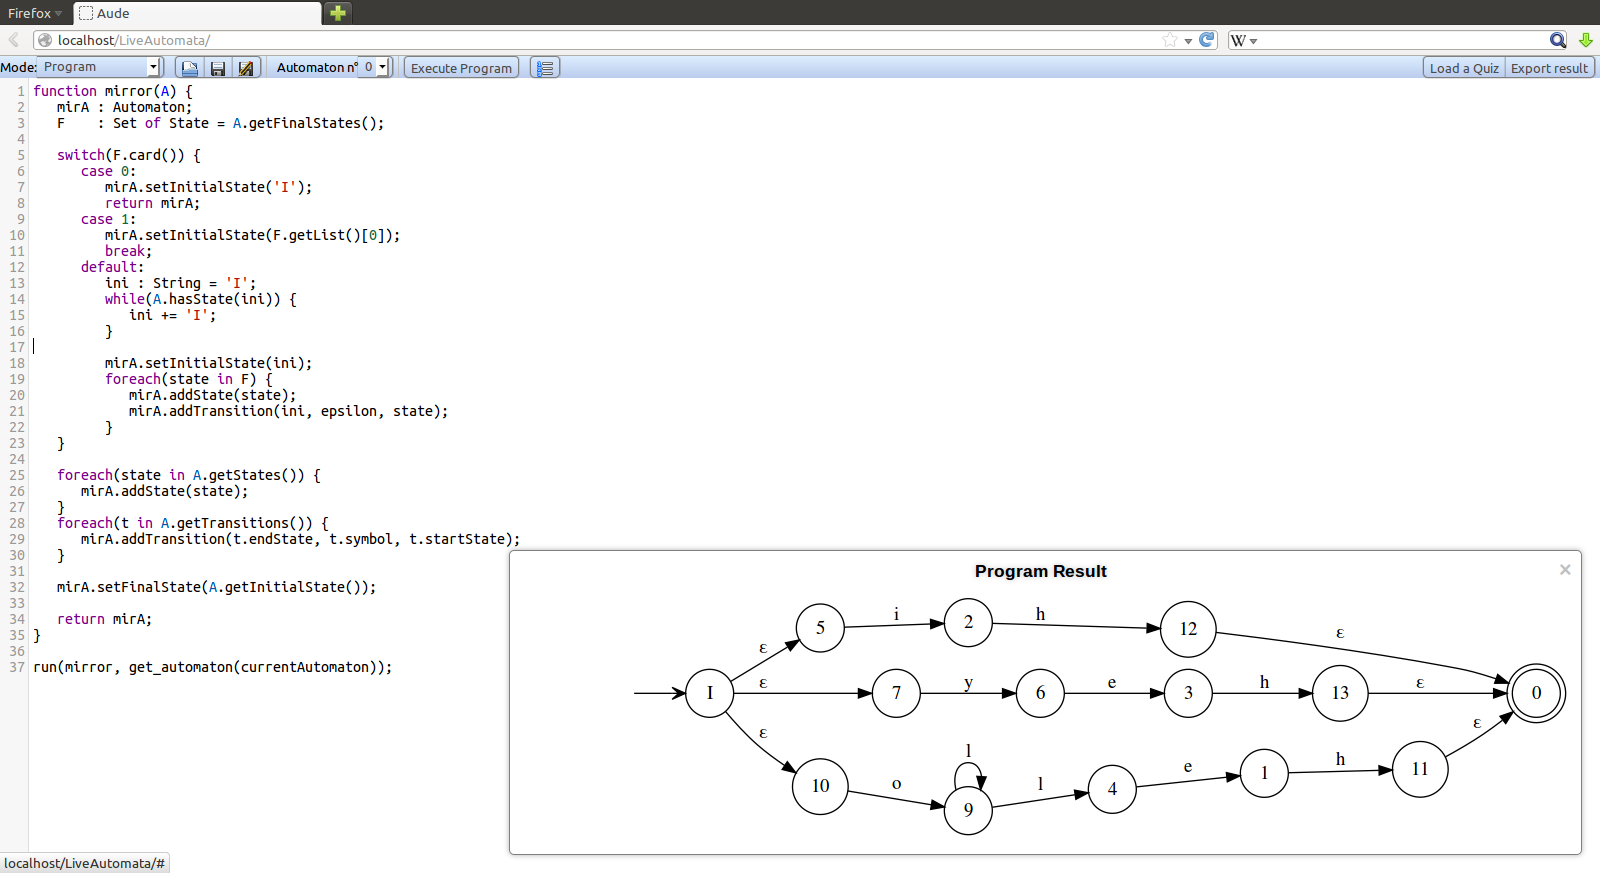
\includegraphics[width=500pt]{{../aude-prog}.png}\caption{Writing algorithms.}\label{aude-prog}\end{figure}


\paragraph{}
Algorithms can take several automata parameters. The user will be asked to choose which automata should be sent to the algorithm when running it.

    \begin{figure}[htb]\centering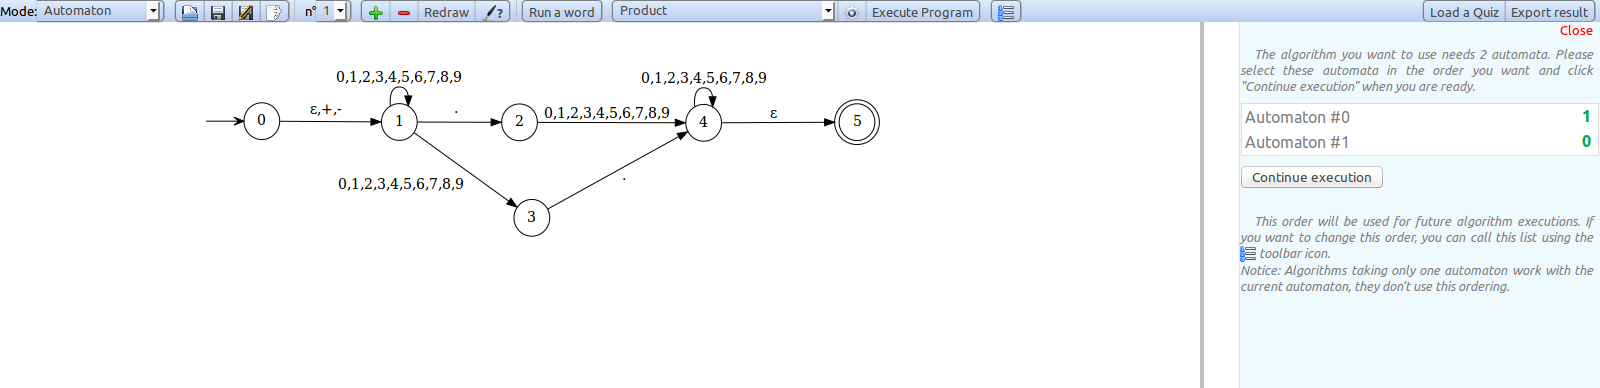
\includegraphics[width=500pt]{{../aude-list-automata}.png}\caption{Choosing which automata should be sent to the algorithm.}\label{aude-list}\end{figure}



\subsection{Running words}

\paragraph{}
Finite state automata are all about word recognition and the execution of a word is probably the most important thing to understand in the automata theory before going any farther. As a result, special care when transmitting the idea of word execution to students must be all the more taken.
The tool features animated word execution and particular attention was taken to make it easy to follow. Students can test words on their drawn and see what path(s) lead to word acceptation or from which state(s) the word was rejected (See figure \ref{word-exec}).

\begin{figure}[htb]\centering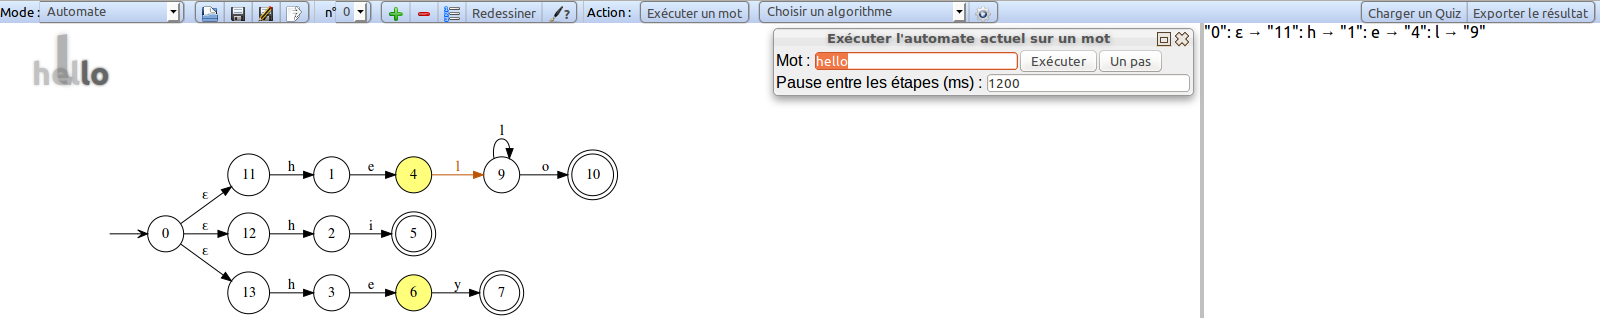
\includegraphics[width=500pt]{{../word-execution}.png}\caption{Word execution.}\label{word-exec}\end{figure}



\subsection{Quizzes}


\paragraph{}
Motivation is important, if not essential, in the process of acquiring knowledge. Interactivity sometimes helps in keeping students motivated and autonomous work can also be sought by a part of the students. \\
We tried to address the issue by implementing a Quiz module in the tool (see figure \ref{aude-quiz}). Teachers (or even students) can write custom quizzes for students so that they can train in autonomy: the tool asks questions, gathers students' responses and tell them what is right and what is wrong.

\paragraph{}
Quizzes can include:

\begin{itemize}
   \item{ mere multiple choice questions, with zero, one or more answers, with any number of possible answers.}
   \item{ questions that ask the user to draw an automaton corresponding to a set of words.}
   \item{ questions that ask the user to draw an automaton corresponding to a language defined by an automaton or a regular expression in the quiz file.}
\end{itemize}

\paragraph{}
The tool supports writing mathematics in the quiz.

\begin{figure}[htb]\centering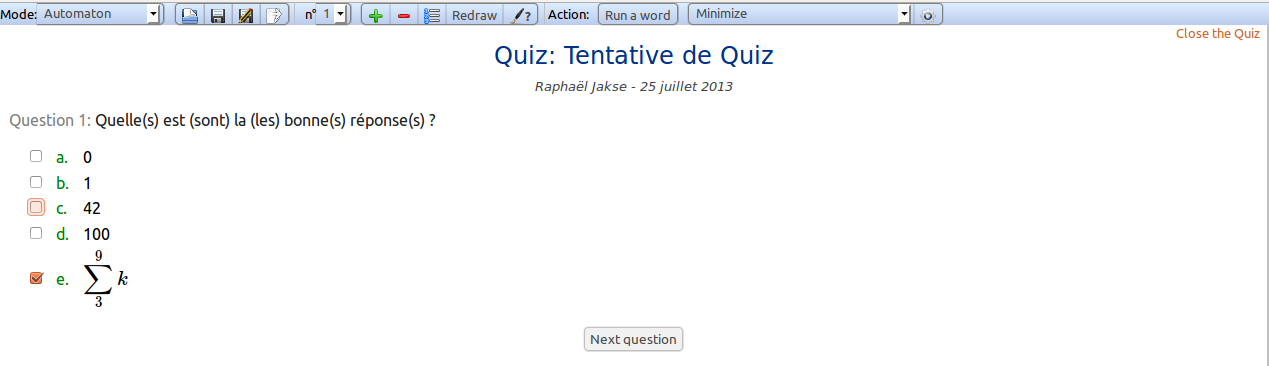
\includegraphics[width=430pt]{{../aude-quiz}.png}\caption{Quiz.}\label{aude-quiz}\end{figure}

\subsection{Automata Theory-compatible Programming Language}
\paragraph{}
The finite state automaton is usually represented by a quintuplet $(Q, \Sigma, \delta, q_0, F)$ where:
\begin{itemize}
   \item{$ Q $ is a \emph{set} of states.}
   \item{$ \Sigma $ is an alphabet. In other words, $ \Sigma $ is a \emph{set} of symbols.}
   \item{$ \delta $ is a transition relation. Put in another way, more precisely, it is a \emph{set} of triplets $(\rm{state}, \rm{symbol}, \rm{state})$.}
   \item{$ q_0 $ is the start state.}
   \item{$ F $ is a \emph{set} of states considered as final, or accepting.}
\end{itemize}

\paragraph{}
The usual definition of the finite state automaton is entirely based and completely depends on sets, and so are automata-related algorithms (see figure~\ref{algo-diff}). As a result, the tool embeds a programming language in which sets are first-class citizens. Instead of writing an entirely new programming language, choice was made to extend Javascript to sets and automata. This implies that students have access to all the features of a widespread generalist programming language as well as features specific to the Automata Theory. See figure~\ref{audejs-ex} to see an implementation of the algorithm~\ref{algo-diff}.

\begin{algorithm}
   \caption{Find differentiable states}
   \label{algo-diff}
   \begin{algorithmic}
      \State \textbf{Input:} $A=(Q, \Sigma, \delta, q_{\rm{init}}, F):$ a deterministic state automaton which all states are accessible.
      \State \textbf{Output:} $D\subseteq Q \times Q$: differentiation relation between states of $ Q $
      \State \textbf{Variables:} $D, D_{\rm{pre}}, X$: sets of state couples
      \State $D \gets \left(F\times (Q \setminus F)\right)$
      \State $D_{\rm{pre}} \gets \{\}$
      \While{$D_{\rm{pre}}\neq D$}
        \State $D_{\rm{pre}}=D$
        \State $X \gets \left\{(p,q) \in Q\: | \: \exists a \in \Sigma, \left(\delta(p,a), \delta(q,a)\right) \in D\right\}$
        \State $D \gets D \cup X$
      \EndWhile
      \State \Return $D$
   \end{algorithmic}
\end{algorithm}

\lstset{language=JavaScript}

\begin{figure}
\label{audejs-ex}
\caption{}
\begin{lstlisting}
function distinguableStates(A) {
   let F     = A.getFinalStates(),
       Q     = A.getStates(),
       Sigma = A.getAlphabet(),
       delta = A.getTransitionFunction(true);

   D     : Set of List = F cross (Q minus F);
   D_pre : Set of List = emptySet;
   X     : Set of List;
   while(D != D_pre) {
      D_pre = D.copy();

      X = emptySet;
      foreach(p in Q) {
         foreach(q in Q) {
            foreach(a in Sigma) {
               if([delta(p, a), delta(q, a)] belongsTo D) {
                  X.add([p, q]);
               }
            }
         }
      }

      D Union= X;
   }
   return D;
}
\end{lstlisting}
\end{figure}
\paragraph{}
Extending a programming language, in our case, means:

\begin{itemize}
   \item{Extending the ``standard library'': adding a class to manipulate sets and a class to manipulate automata.}
   \item{Modifying the grammar of the language: adding features like set manipulations and iteration.}
\end{itemize}

\paragraph{}
Concretely, the tool embeds a function which maps a code written in our programming language to a pure Javascript code. This Javascript code can then be executed in any Javascript-compatible Web browser.
The mapping is done with the following constraints:
\begin{itemize}
   \item{ $ n $\textsuperscript{th} line  of the generated code must correspond to the $ n $\textsuperscript{th}  line of the input code, for accuracy in error reporting}
   \item{ The generated code must be identical to the input code if the input code is pure Javascript.}
\end{itemize}

\paragraph{}
Since sets look like Javascript blocks of code, transformations must not be done inside strings, and some transformations can be nested, regular expressions are not sufficient to handle the translation.

\DefineShortVerb{\#}
\SaveVerb{v1}#foreach(i in object) { ... }#
\SaveVerb{v3}#varname : Type#
\SaveVerb{v4}#var varname = new Type#
\UndefineShortVerb{\#}

\lstset{numbers=none, frame=none}

\newsavebox\foreachinput
\begin{lrbox}{\foreachinput}
\begin{minipage}{0.5\textwidth}
 \begin{lstlisting}
foreach(e in mySet) {
  if(e == {1,2,3}) {
   break; // we found our triplet
  }
  else if(e instanceof Set) { // if e is a Set
    try{(e).forEach(function(f ) {
      if( contains(e, epsilon)) {
        throw 0; //we found epsilon
      }
    }
  )}catch(e){if(e instanceof Error){throw e}else if(!(e === StopIteration)){throw e;}}}

  if(  Audescript.eq(e, new Set())) {
     throw -1; // we found the empty set. Stopping the execution.
  }
}

// ...
)}catch(e){if(e instanceof Error){throw e}else if(!(e === StopIteration)){return e;}}
 \end{lstlisting}
\end{minipage}
\end{lrbox}


\newsavebox\foreachgenerated
\begin{lrbox}{\foreachgenerated}
\begin{minipage}{0.5\textwidth}
 \begin{lstlisting}
try{(object).forEach(function (i ) {

}
)}catch (e) {if (e instanceof audescript.ThrowValue) {throw e.v;}else if (e instanceof audescript.ReturnValue) {return e.v;}}
 \end{lstlisting}
\end{minipage}
\end{lrbox}

\noindent\begin{tabularx}{\linewidth}{|*{2}{X|}}
\hline
{\bfseries  Input code                              } & {\bfseries  Generated code             }\tabularnewline
\hline
 \UseVerb{v1}  & \usebox\foreachgenerated \tabularnewline
\hline
 \UseVerb{v3}                &  \UseVerb{v4}       \tabularnewline
\hline
\end{tabularx}

\paragraph{}
These transformations must not be done inside string literals, {\itshape object} in \lstinline!foreach! can contain parenthesis, the variable declaration can hold a initialization value, set literals look very similar to blocks of codes, \lstinline!foreach! can be nested so a need to match curly brackets appears, \lstinline!break! and \lstinline!return! statement must be transformed inside \lstinline!foreach! loop, etc. Manipulated languages are not {\itshape regular}\footnote{a language is regular iff it can be described with a regular expression. Rules like “there is the same number of opening and closing parenthesis” make a language not regular.} and transformations are not that trivial eventually. As a consequence, another method needs to be used, the code must be parsed more subtly.

\paragraph{}
A project like \href{http://zaach.github.io/jison/}{Jison}, which is a parser like \href{http://www.gnu.org/software/bison/}{Bison} might have been used\footnote{See \href{http://cjihrig.com/blog/creating-a-javascript-parser/}{http://cjihrig.com/blog/creating-a-javascript-parser/} for an implementation of a Javascript parser with Jison}. However, handwriting the parser was chosen in order to keep whitespace characters intact, to have full control over optional semicolons (if a semicolon was not written by the programmer, the semicolon should not appear in the generated code) and to handle ambiguities between regular expression tokens (which begin with \lstinline!/!) and division operators (\lstinline!/!, \lstinline!/=!) easily. Handwriting the parser also seemed to be a more efficient and straightforward solution here because transformations can be made without generating any abstract syntax tree. Moreover, this lets write a quite flexible parser, validation being delegated to the actual Javascript engine, which already has a good error reporting system.

\section{Comparison with other tools}

\paragraph{}
Like most tools of the domain, the tool gives the ability to the user to draw automata. However, unlike its friends, the user has more freedom in {\em choosing the shape of the transitions}, though Visual Automata Simulator is great for this, and thanks to the tight integration of Graphviz, automata can be {\em (re)drawn automatically} and have a {\em familiar look}.
   
   
\paragraph{}
Like most others tools, the program comes with basic common algorithms related to automata. However, it comes with {\em far more algorithms} than its friends and {\em lets the user write its own algorithms easily}, providing a language close to Javascript with sets as first-class citizens, which makes it suitable for manipulation of automata.

   
\paragraph{}
The program is designed with the user in mind: everything is thought to be the more pleasant and natural possible, appearance not being set aside. An example of this is the graphical execution of a word: current states are seen in yellow, transitions being taken right now are brown and current final states are green. If a word runs out of the automaton, its states are drawn in red. The execution can be made {\em step by step} or not and animations were designed to ease the visualization of the execution.

   
\paragraph{}
What also make the program stand out is the Quiz Feature: it gives the ability to teachers and students to {\em write quiz for students} and these quizzes are run by the tool, using its automata manipulation capabilities. Questions of the quiz can be mere multiple choices questions as well as asking the user to write automata or regular expressions.
   
   
\paragraph{}
Another thing that can be said is that unlike others tools, this one is written with web technologies, which makes the program usable without any installation and will make the port on tablets easy. Thanks to web technologies, the program should work on any desktop operating system, provided a recent browser is installed, and the support for mobile operating systems should follow quickly.

   
\newpage
   
\paragraph{}
The following table\footnote{Icons in the table come from the Oxygen theme: \href{http://www.oxygen-icons.org/}{http://www.oxygen-icons.org/}} compares Aude with some other tools of the domain.

      \noindent\begin{tabularx}{\linewidth}{|*{6}{X|}}
\hline
{\bfseries  Feature                    } & {\bfseries  Aude         } & {\bfseries  jFAST} & {\bfseries jFLAP  } & {\bfseries  Visual Automata Simulator (VAS) } & {\bfseries Finite Automata Tool (FAT)}\tabularnewline
\hline
 Finite-state automata        &  
\includegraphics[height=14pt]{{../dialog-ok-apply}.png}            &  
\includegraphics[height=14pt]{{../dialog-ok-apply}.png}    &  
\includegraphics[height=14pt]{{../dialog-ok-apply}.png}     &  
\includegraphics[height=14pt]{{../dialog-ok-apply}.png}                        &  
\includegraphics[height=14pt]{{../dialog-ok-apply}.png}\tabularnewline
\hline
 Turing Machine               &  
\includegraphics[height=14pt]{{../edit-delete}.png}             &  
\includegraphics[height=14pt]{{../edit-delete}.png}     &  
\includegraphics[height=14pt]{{../dialog-ok-apply}.png}     &  
\includegraphics[height=14pt]{{../dialog-ok-apply}.png}                        &  
\includegraphics[height=14pt]{{../edit-delete}.png}\tabularnewline
\hline
 Mealy Machine                &  
\includegraphics[height=14pt]{{../edit-delete}.png}             &  
\includegraphics[height=14pt]{{../edit-delete}.png}     &  
\includegraphics[height=14pt]{{../dialog-ok-apply}.png}     &  
\includegraphics[height=14pt]{{../edit-delete}.png}                         &  
\includegraphics[height=14pt]{{../edit-delete}.png}\tabularnewline
\hline
 More Machine                 &  
\includegraphics[height=14pt]{{../edit-delete}.png}             &  
\includegraphics[height=14pt]{{../edit-delete}.png}     &  
\includegraphics[height=14pt]{{../dialog-ok-apply}.png}     &  
\includegraphics[height=14pt]{{../edit-delete}.png}                         &  
\includegraphics[height=14pt]{{../edit-delete}.png}\tabularnewline
\hline
 Pushdown automaton           &  
\includegraphics[height=14pt]{{../edit-delete}.png}             &  
\includegraphics[height=14pt]{{../edit-delete}.png}     &  
\includegraphics[height=14pt]{{../dialog-ok-apply}.png}     &  
\includegraphics[height=14pt]{{../edit-delete}.png}                         &  
\includegraphics[height=14pt]{{../edit-delete}.png}\tabularnewline
\hline
 Grammar Manipulation         &  
\includegraphics[height=14pt]{{../edit-delete}.png}             &  
\includegraphics[height=14pt]{{../edit-delete}.png}     &  
\includegraphics[height=14pt]{{../dialog-ok-apply}.png}     &  
\includegraphics[height=14pt]{{../edit-delete}.png}                         &  
\includegraphics[height=14pt]{{../edit-delete}.png}  \tabularnewline
\hline
 Draw automata                &  
\includegraphics[height=14pt]{{../dialog-ok-apply}.png}            &  
\includegraphics[height=14pt]{{../dialog-ok-apply}.png}    &  
\includegraphics[height=14pt]{{../dialog-ok-apply}.png}     &  
\includegraphics[height=14pt]{{../dialog-ok-apply}.png}                        &  
\includegraphics[height=14pt]{{../edit-delete}.png}\tabularnewline
\hline
 Regular expression to FSA    &  
\includegraphics[height=14pt]{{../dialog-ok-apply}.png}            &  
\includegraphics[height=14pt]{{../edit-delete}.png}     &  
\includegraphics[height=14pt]{{../dialog-ok-apply}.png}     &  
\includegraphics[height=14pt]{{../edit-delete}.png}                         &  
\includegraphics[height=14pt]{{../edit-delete}.png}\tabularnewline
\hline
 Run a word                   &  
\includegraphics[height=14pt]{{../dialog-ok-apply}.png}            &  Complete DFA only  &  
\includegraphics[height=14pt]{{../dialog-ok-apply}.png}  &  no epsilon transition  &  
\includegraphics[height=14pt]{{../edit-delete}.png}\tabularnewline
\hline
 Apply basic algorithms       &  
\includegraphics[height=14pt]{{../dialog-ok-apply}.png}            &  
\includegraphics[height=14pt]{{../edit-delete}.png}     &  Determinization, minimization, completion  &   Determinization  &  Union, Intersection, Complementation, Minimization, Determinization\tabularnewline
\hline
 Combine two automata         &  \includegraphics[height=14pt]{{../edit-delete}.png}             &  \includegraphics[height=14pt]{{../edit-delete}.png}     &  \includegraphics[height=14pt]{{../dialog-ok-apply}.png}     &  \includegraphics[height=14pt]{{../edit-delete}.png}                        &  \includegraphics[height=14pt]{{../edit-delete}.png}\tabularnewline
\hline
 Quiz                         &  \includegraphics[height=14pt]{{../dialog-ok-apply}.png}            &  \includegraphics[height=14pt]{{../edit-delete}.png}     &  \includegraphics[height=14pt]{{../edit-delete}.png}      &  \includegraphics[height=14pt]{{../edit-delete}.png}                        &  \includegraphics[height=14pt]{{../edit-delete}.png}\tabularnewline
\hline
 Games                        &  \includegraphics[height=14pt]{{../edit-delete}.png}             &  \includegraphics[height=14pt]{{../edit-delete}.png}     &  Pumping Lemma  &  \includegraphics[height=14pt]{{../edit-delete}.png}                 &  \includegraphics[height=14pt]{{../edit-delete}.png}\tabularnewline
\hline
 User's algorithms            &  \includegraphics[height=14pt]{{../dialog-ok-apply}.png}            &  \includegraphics[height=14pt]{{../edit-delete}.png}     &  \includegraphics[height=14pt]{{../edit-delete}.png}      &  \includegraphics[height=14pt]{{../edit-delete}.png}                        &  \includegraphics[height=14pt]{{../edit-delete}.png}\tabularnewline
\hline
 Consult built-in algorithms  &  \includegraphics[height=14pt]{{../dialog-ok-apply}.png}            &  \includegraphics[height=14pt]{{../edit-delete}.png}     &  \includegraphics[height=14pt]{{../edit-delete}.png}      &  \includegraphics[height=14pt]{{../edit-delete}.png}                        &  \includegraphics[height=14pt]{{../edit-delete}.png}\tabularnewline
\hline
 Automatic automaton drawing  &  \includegraphics[height=14pt]{{../dialog-ok-apply}.png}            &  \includegraphics[height=14pt]{{../edit-delete}.png}     &  \includegraphics[height=14pt]{{../edit-delete}.png}      &  \includegraphics[height=14pt]{{../edit-delete}.png}                        &  \includegraphics[height=14pt]{{../edit-delete}.png}\tabularnewline
\hline
 Automaton code input         &  \includegraphics[height=14pt]{{../dialog-ok-apply}.png}            &  \includegraphics[height=14pt]{{../edit-delete}.png}     &  \includegraphics[height=14pt]{{../edit-delete}.png}      &  \includegraphics[height=14pt]{{../edit-delete}.png}                        &  \includegraphics[height=14pt]{{../dialog-ok-apply}.png}\tabularnewline
\hline
 Run online                   &  \includegraphics[height=14pt]{{../dialog-ok-apply}.png}            &  Java RE  &  Java RE  &  Java RE  &  Java RE\tabularnewline
\hline
 Requires                     &  A Web browser  &  Java   &  Java    &  Java                      &  Java\tabularnewline
\hline
\end{tabularx}


\section{Using the tool}

\subsection{Running Aude}
\paragraph{}
The easiest way to run Aude is to use it online with any recent browser (Internet Explorer is not tested often, it is recommended to use another browser. Opera prior to version 15 and Konqueror/KHTML are not supported).

\paragraph{}
Running Aude off-line is also supported. The most recommended way to do this is to open the \verb!index.html! file in Firefox / Iceweasel or Arora. You can also use Chromium/Google Chrome and Opera 15+, but the \verb!--allow-file-access-from-files! command line switch is needed when launching the browser. Midori and epiphany are not supported for off-line usage yet. Safari and Internet Explorer are not tested for offline usage.

\paragraph{}
The \verb!aude! shell script can be used on Unix systems to run Aude, it should take care of command line switches and will use the \verb!BROWSER! variable environment if it is set, or choose a suitable browser otherwise.

\subsection{Drawing an automaton}

\paragraph{}
To draw an automaton, you should be in the "Automaton" mode, which is the default mode when you run Aude. You can click on the "plus" button if there is already an automaton and you want to begin a new one. You can also click on the "minus" button if you want to discard the current automaton.

\paragraph{}
Drawing automata is done by using a mouse and a keyboard. Others input devices are not supported yet, though a workaround (on a tablet for example) would be to input automata using the "automaton code" mode and then to move states in the "Automaton" mode. The more frequently an action is likely to be taken, the simpler the steps to perform it.

\paragraph{}
To {\bfseries add a state}, double-click on the drawing area. The state gets a default name and is set to initial if it is the only state present. You can change the name of the state by double-clicking on it.

\paragraph{}
If you want to want to {\bfseries make a state accepting}, right-click on it. Accepting states are double-circled. To make a state non accepting, right-click on it.

\paragraph{}
To {\bfseries change the initial state}, control-right click on the new initial state.

\paragraph{}
If you want to {\bfseries add a transition}, shift+click on the state from which the transition should begin, and click on the destination state. You can release shift and/or the button of the mouse if you wish, though it is not mandatory.

You will be asked to enter the symbols of the transition separated by commas. To {\bfseries modify the symbols} of a transition, double-click on them.

See the note on epsilon to know how to input epsilons.

\paragraph{}
At any time, you can click on the help button ({\bfseries \includegraphics[width=10pt]{{draw-brush}.png}?}) to {\bfseries get a reminder on how to perform an action}.

\paragraph{}
You can {\bfseries change the shape of a transition} by clicking on the head of the arrow and moving the control points. To {\bfseries make a transition straight}, shift+click on the head of the arrow.

\paragraph{}
You can {\bfseries zoom / unzoom} by using the wheel. The area is zoomed at the place where the cursor of the mouse is.

\paragraph{}
If you want your automaton to be {\bfseries automatically reorganized} (using the Graphviz engine), you can click on the "redraw" button.

\paragraph{}
{\bfseries To delete a transition}, control-click on the head of its arrow or on its symbol list. {\bfseries To delete a state}, control-click on it as well.

\subsection{Entering an automaton}

\paragraph{}
Complementary to drawing, you can input an automaton by issuing its code in the Aude interface. Select the "Automaton Code" mode at the top-left side of Aude.

The code of an automaton is composed of: a non-empty list of states begining with the initial state, a list of accepting states, and a list of transition. A SVG representation can be given between \verb!<representation type='image/svg+xml'>! and \verb!</representation>!, after the list of transitions. For each list, each element has its own line (one element per line), and lists are separated by an empty line (even in case of empty lists). A transition is given by an origin state, a symbol and a destination state (in this order), separated by spaces. See the note on epsilon to know how to handle epsilons.

\subsection{Note on epsilon}
\paragraph{}
When giving the symbols of a transition, you might need to use epsilon. The special symbol \textit{epsilon}, which is the empty symbol, can be given with the epsilon character or with a \verb!e! escaped with a backslash (\verb!\e!). If you really need your automaton to recognize the real epsilon character (non-empty character), surround it with double-quotes~: (\verb!"\e"!).

\subsection{Saving, loading, exporting an automaton}
\paragraph{}
You can save and load automata. Click on the load/save/save as button when you are in the "Automaton" or the "Automaton code" mode.

You can also export an automaton in the SVG or the DOT (Graphviz) formats by clicking the export button, in order to use them in documents. The DOT format won't keep your custom placements. SVG pictures can be exported in the EPS format in order to be used in LaTeX documents or can be used as is in HTML documents (check browser SVG compatibilities if you need to support old browsers). You can also convert SVG to any other image format (like PNG, JPG, etc). SVG and EPS are vector formats, so you can zoom infinitely without loosing quality, we therefore recommend you to use them whenever possible.

\subsection{Run a word}
\paragraph{}
You can test a word against an automaton and visualize the execution. Click on "Run a word" in the "Automaton" mode when you have your automaton done; a window appear. In this window, input the word you want to test, and click on "execute" or "one step", if you want the execution run without interruption or if you can to control the execution. The execution is detailed in a textual format in the "result" part of Aude. Closing the windows causes the execution to end.

\subsection{Running an algorithm}
\paragraph{}
Aude comes with predefined algorithm. Most algorithms work on an automaton. When you have an automaton ready in the "automaton" or "automaton code" mode, choose an algorithm and click on "run". The result will appear at the right side of aude. If the result is an automaton, you can save it in the Aude format by clicking on the "export the result" button. You can also edit it by clicking on he "this automaton in the editor" button. In this case, the current automaton is kept and a new number is assigned to the result in the editor.

\paragraph{}
Some algorithms need more than one automaton. For example, automata equivalence is an algorithm which needs two automata. In this case, it is necessary to select the automata which are to give to the algorithm and to specify the order in which they are given.

\paragraph{}
First, automata which are to give must be loaded in the program. You could have just drawn them, or opened them from files. What is important is that they have a number.

\paragraph{}
Then, click on the "choose automata parameters" icon~: \includegraphics[width=10pt]{{format-list-ordered}.png}. Click on the automata which are to give to the algorithm in the right order. Clicking on an automaton another time deletes it from the list. When you are ready, you can run the algorithm as usual.

\subsection{Load or write a program}
\paragraph{}
First, choose the "Program" mode. From there, you can open an existing program with the "open" button. You can run the program by clicking on the "run program" button. This button also appears in "automaton" and "automaton code" modes when there is a program in the "program" mode.

\paragraph{}
Programs are written using the Audescript programming language. This language is derived from Javascript. The main differences are:

\begin{itemize}
	\item{Audescript has set literals, like \verb!{1,2,3}! or \verb!{"Hello", "world"}!}
	\item{Audescript has set operators, like \verb!minus!, \verb!union!, \verb!cross!, \verb!inter!, \verb!symDiff!}
	\item{Audescript lets you type variables, like in \verb!a : int!, \verb!a : Automaton!, \verb!l : Array!, \verb!s : Set of String = {"hello", "world"}!, functions and function parameters like in \verb!function sum(a : int, b : int) : int { return a + b;}!. Type checking is done at runtime.}
\end{itemize}

\paragraph{}
For examples of programs written in Audescript, you can take a look at Aude's predefined algorithms and tests present in the \verb!tests! folder of Aude.

\subsection{Load a Quiz}
\paragraph{}
Aude has an experimental Quiz module. To load a quiz, click on the "Load a Quiz" button and choose a quiz. If you want to write a quiz, you can take a look at the "quiz" folder of Aude for an example of Quiz.

\paragraph{}
What is supported by the quiz module is multiple choice questions, drawing an automaton which must recognize a language given by a set of words, an equivalent automaton or a regular expression. The quiz ends by a recap giving what was correctly, incorrectly or partially answered.

\subsection{Using the Audescript interpreter}
Aude comes with a standalone Audescript interpreter which depends on Node.js. It was only tested on Linux so far. In order to run the interpreter, in a terminal, move to the Aude directory and run:

\begin{verbatim}
./audescript yourprogram.ajs parameters...
\end{verbatim}

Audescript can also act as an interactive shell:

\begin{verbatim}
./audescript
\end{verbatim}

File redirections are also supported:

\begin{verbatim}
./audescript < file.ajs
\end{verbatim}

It is possible to install Aude (with make install for example). In this case, you can launch the interpreter from everywhere and leave the "./" part of the commands.


\section{Future work}

\section{Conclusion}


\end{sloppypar}
\end{document}
